%!TeX root=../wowtop.tex

\ArtChapter[The Cylinder Opens]{4head}


\lettrine[lines=4,findent=2pt]{W}{hen} I returned to the common the sun was setting. Scattered groups were hurrying from the direction of Woking, and one or two persons were returning. The crowd about the pit had increased, and stood out black against the lemon yellow of the sky—a couple of hundred people, perhaps. There were raised voices, and some sort of struggle appeared to be going on about the pit. Strange imaginings passed through my mind. As I drew nearer I heard Stent's voice:

»Keep back! Keep back!«

A boy came running towards me.

»It's a-movin',« he said to me as he passed; »a-screwin' and a-screwin' out. I don't like it. I'm a-goin' 'ome, I am.«

I went on to the crowd. There were really, I should think, two or three hundred people elbowing and jostling one another, the one or two ladies there being by no means the least active.

»He's fallen in the pit!« cried some one.

»Keep back!« said several.

The crowd swayed a little, and I elbowed my way through. Every one seemed greatly excited. I heard a peculiar humming sound from the pit.

»I say!« said Ogilvy; »help keep these idiots back. We don't know what's in the confounded thing, you know!«

I saw a young man, a shop assistant in Woking I believe he was, standing on the cylinder and trying to scramble out of the hole again. The crowd had pushed him in.

The end of the cylinder was being screwed out from within. Nearly two feet of shining screw projected. Somebody blundered against me, and I narrowly missed being pitched onto the top of the screw. I turned, and as I did so the screw must have come out, for the lid of the cylinder fell upon the gravel with a ringing concussion. I stuck my elbow into the person behind me, and turned my head towards the Thing again. For a moment that circular cavity seemed perfectly black. I had the sunset in my eyes.

I think everyone expected to see a man emerge—possibly something a little unlike us terrestrial men, but in all essentials a man. I know I did. But, looking, I presently saw something stirring within the shadow: greyish billowy movements, one above another, and then two luminous disks—like eyes. Then something resembling a little grey snake, about the thickness of a walking stick, coiled up out of the writhing middle, and wriggled in the air towards me—and then another.

A sudden chill came over me. There was a loud shriek from a woman behind. I half turned, keeping my eyes fixed upon the cylinder still, from which other tentacles were now projecting, and began pushing my way back from the edge of the pit. I saw astonishment giving place to horror on the faces of the people about me. I heard inarticulate exclamations on all sides. There was a general movement backwards. I saw the shopman struggling still on the edge of the pit. I found myself alone, and saw the people on the other side of the pit running off, Stent among them. I looked again at the cylinder, and ungovernable terror gripped me. I stood petrified and staring.

A big greyish rounded bulk, the size, perhaps, of a bear, was rising slowly and painfully out of the cylinder. As it bulged up and caught the light, it glistened like wet leather.

\begin{figure}[p]
	\centering
	
\includegraphics[width=\linewidth]{4opens}
	\caption[A big greyish rounded bulk was rising out of the cylinder]{A big greyish rounded bulk was rising slowly and painfully out of the cylinder}
\end{figure}

Two large dark-coloured eyes were regarding me steadfastly. The mass that framed them, the head of the thing, was rounded, and had, one might say, a face. There was a mouth under the eyes, the lipless brim of which quivered and panted, and dropped saliva. The whole creature heaved and pulsated convulsively. A lank tentacular appendage gripped the edge of the cylinder, another swayed in the air.

Those who have never seen a living Martian can scarcely imagine the strange horror of its appearance. The peculiar V-shaped mouth with its pointed upper lip, the absence of brow ridges, the absence of a chin beneath the wedgelike lower lip, the incessant quivering of this mouth, the Gorgon groups of tentacles, the tumultuous breathing of the lungs in a strange atmosphere, the evident heaviness and painfulness of movement due to the greater gravitational energy of the earth—above all, the extraordinary intensity of the immense eyes—were at once vital, intense, inhuman, crippled and monstrous. There was something fungoid in the oily brown skin, something in the clumsy deliberation of the tedious movements unspeakably nasty. Even at this first encounter, this first glimpse, I was overcome with disgust and dread.

Suddenly the monster vanished. It had toppled over the brim of the cylinder and fallen into the pit, with a thud like the fall of a great mass of leather. I heard it give a peculiar thick cry, and forthwith another of these creatures appeared darkly in the deep shadow of the aperture.

I turned and, running madly, made for the first group of trees, perhaps a hundred yards away; but I ran slantingly and stumbling, for I could not avert my face from these things.

There, among some young pine trees and furze bushes, I stopped, panting, and waited further developments. The common round the sand-pits was dotted with people, standing like myself in a half-fascinated terror, staring at these creatures, or rather at the heaped gravel at the edge of the pit in which they lay. And then, with a renewed horror, I saw a round, black object bobbing up and down on the edge of the pit. It was the head of the shopman who had fallen in, but showing as a little black object against the hot western sun. Now he got his shoulder and knee up, and again he seemed to slip back until only his head was visible. Suddenly he vanished, and I could have fancied a faint shriek had reached me. I had a momentary impulse to go back and help him that my fears overruled.

Everything was then quite invisible, hidden by the deep pit and the heap of sand that the fall of the cylinder had made. Anyone coming along the road from Chobham or Woking would have been amazed at the sight—a dwindling multitude of perhaps a hundred people or more standing in a great irregular circle, in ditches, behind bushes, behind gates and hedges, saying little to one another and that in short, excited shouts, and staring, staring hard at a few heaps of sand. The barrow of ginger beer stood, a queer derelict, black against the burning sky, and in the sand-pits was a row of deserted vehicles with their horses feeding out of nosebags or pawing the ground.

\begin{figure}[b!]
\centering
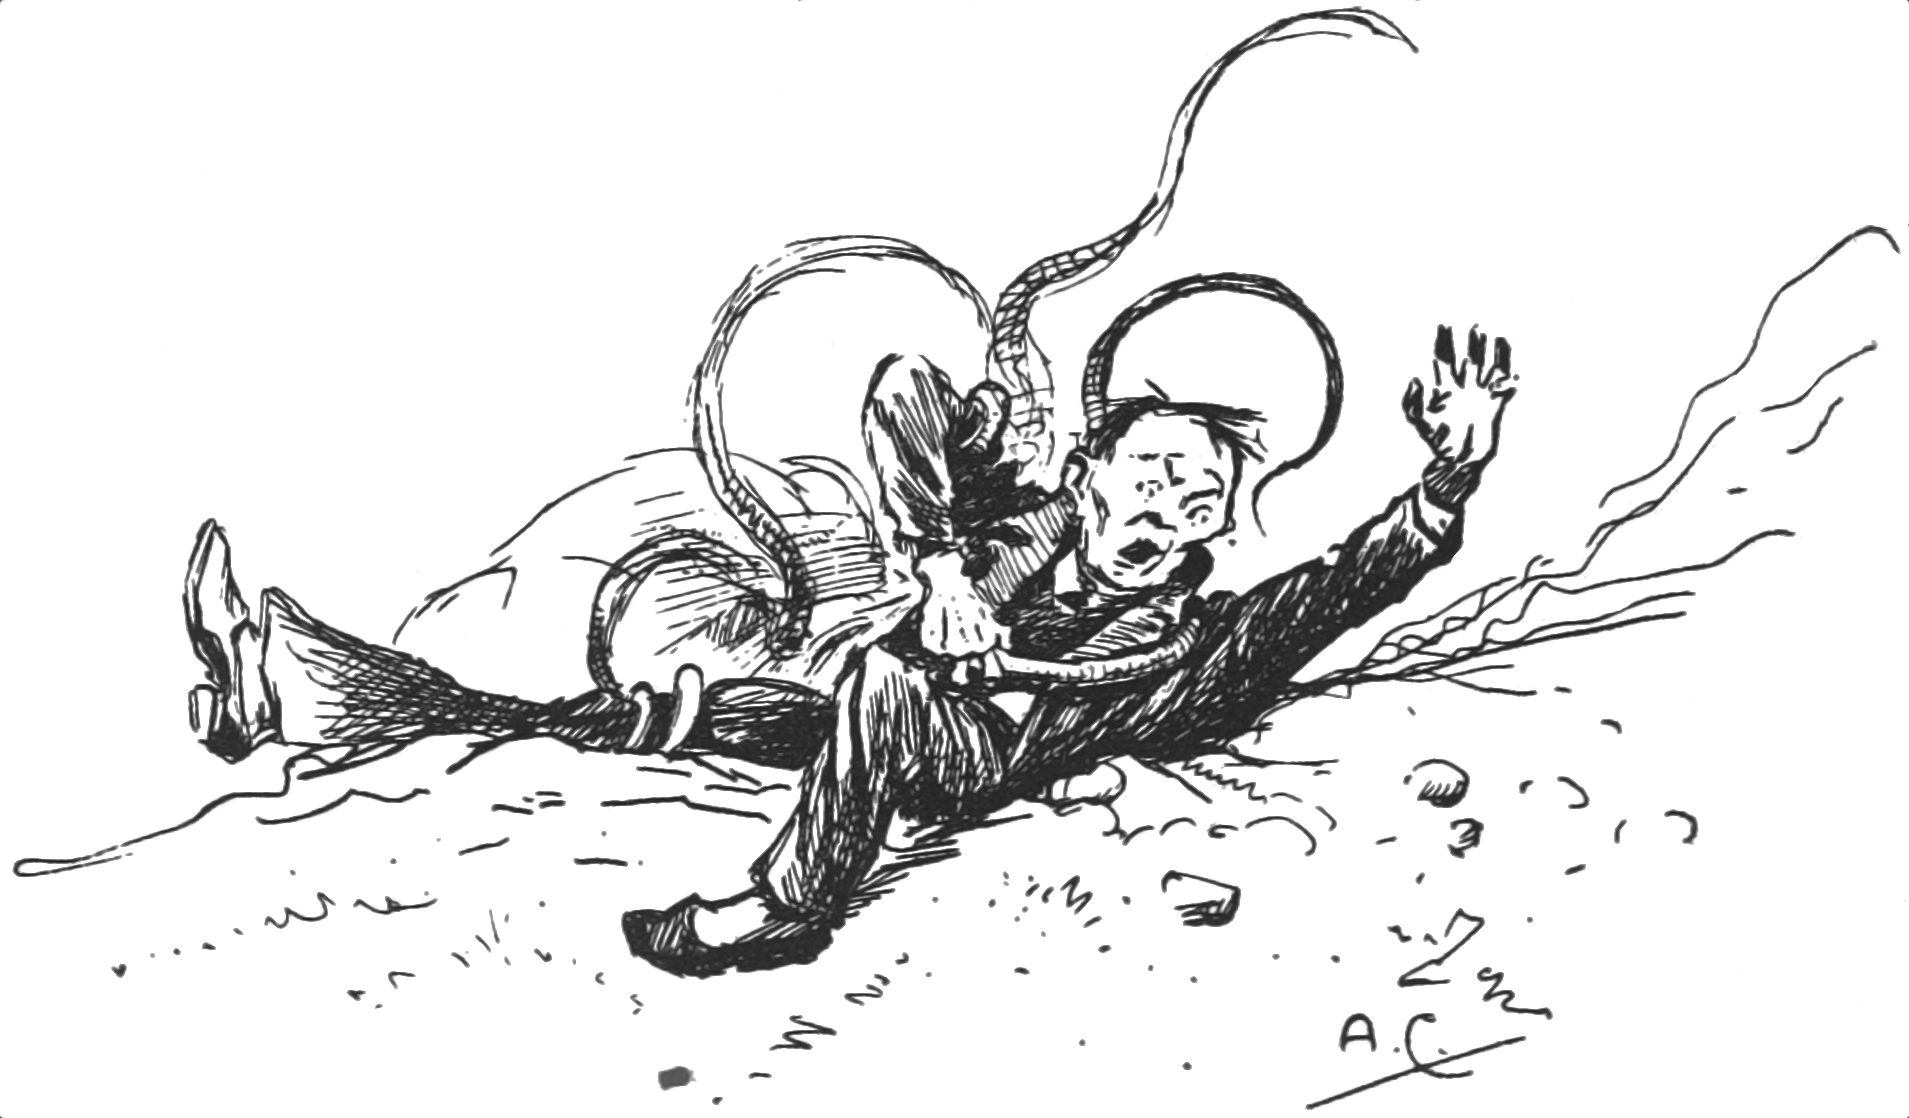
\includegraphics[width=0.7\textwidth]{4tailpiece}
%\captionlistentry{Tailpiece to Chapter \thechapter}
\end{figure}